\documentclass[./PianoDiProgetto.tex]{subfiles}
\begin{document}
\section{Pianificazione}
  Elenchiamo qui di seguito le caratteristiche e le durate di ogni periodo. Nella decisione dei tempi sono stati tenuti in considerazione e si sono cercati di mitigare i rischi relativi alle tempistiche.
	\subsection{\PerAR{} (AR)}
  \textbf{Periodo: dal 2016-12-10 al 2017-01-11}

  Questo periodo comincia con il primo incontro del gruppo e termina con la scadenza della consegna riguardante la \textbf{Revisione dei requisiti}.

  È composto principalmente dalle seguenti attività:
  \begin{enumerate}
		\item \textbf{Scelta degli strumenti}: verranno scelti gli strumenti che saranno utilizzati per la stesura dei documenti e per il supporto. La scelta degli strumenti sarà incrementale nel corso del \gl{progetto};
		\item \textbf{Stesura delle Norme di progetto}: dopo aver scelto i primi strumenti per la produzione di documentazione sarà possibile iniziare la stesura delle \NPdocRR. Questo documento sarà utilizzato indipendentemente dal \gl{capitolato} che verrà preso in appalto, e sarà steso in modo incrementale via via che nuove norme verranno definite;
		\item \textbf{Stesura documentazione}: una volta definiti norme e strumenti per la scrittura di un documento, è possibile iniziare la stesura della documentazione;
    \begin{itemize}
      \item \textbf{Analisi dei Requisiti}: viene effettuata l'analisi dei requisiti, in cui vengono individuati i principali requisiti del progetto, che vengono poi inseriti nel documento \ARdocRR. Verranno organizzati degli incontri col \gl{proponente}, sia prima che durante la stesura di questo documento, per consolidare i requisiti stesi e per chiarire eventuali dubbi sui requisiti da aggiungere;
      \item \textbf{Studio di Fattibilità}: vengono valutati pro e contro di tutti i capitolati proposti e viene redatto il documento \SFdocRR. Viene quindi scelto il capitolato da sviluppare;
      \item \textbf{Piano di Progetto}: viene steso il documento \PPdocRR, il quale regolerà le attività del gruppo;
      \item \textbf{Piano di qualifica}: si stende il documento \PQdocRR per fissare gli standard di qualità ed in che modo il gruppo si prefigge di raggiungerli;
      \item \textbf{Glossario}: viene creato il file incrementale "terminiGlossario.txt" e steso in modo automatico il documento \GldocRR;
      \item \textbf{Lettera di Presentazione}: si scrive la lettera in cui si dichiara l'interesse del gruppo a partecipare alla gara di appalto;
      \item \textbf{Analisi preliminare degli \gl{SDK} dei principali assistenti virtuali}: gli \ANP{} analizzeranno gli SDK dei principali assistenti virtuali, dotati di intelligenza artificiale, presenti sul mercato, e scriveranno il documento esterno \textit{"AnalisiSDK v1.0.0"} in cui verrà effettuato il confronto tra  essi.
    \end{itemize}
  \end{enumerate}
  \newpage
  \subsubsection{Diagramma di Gantt - \PerAR}
    \begin{figure}[!h]
    \centering
    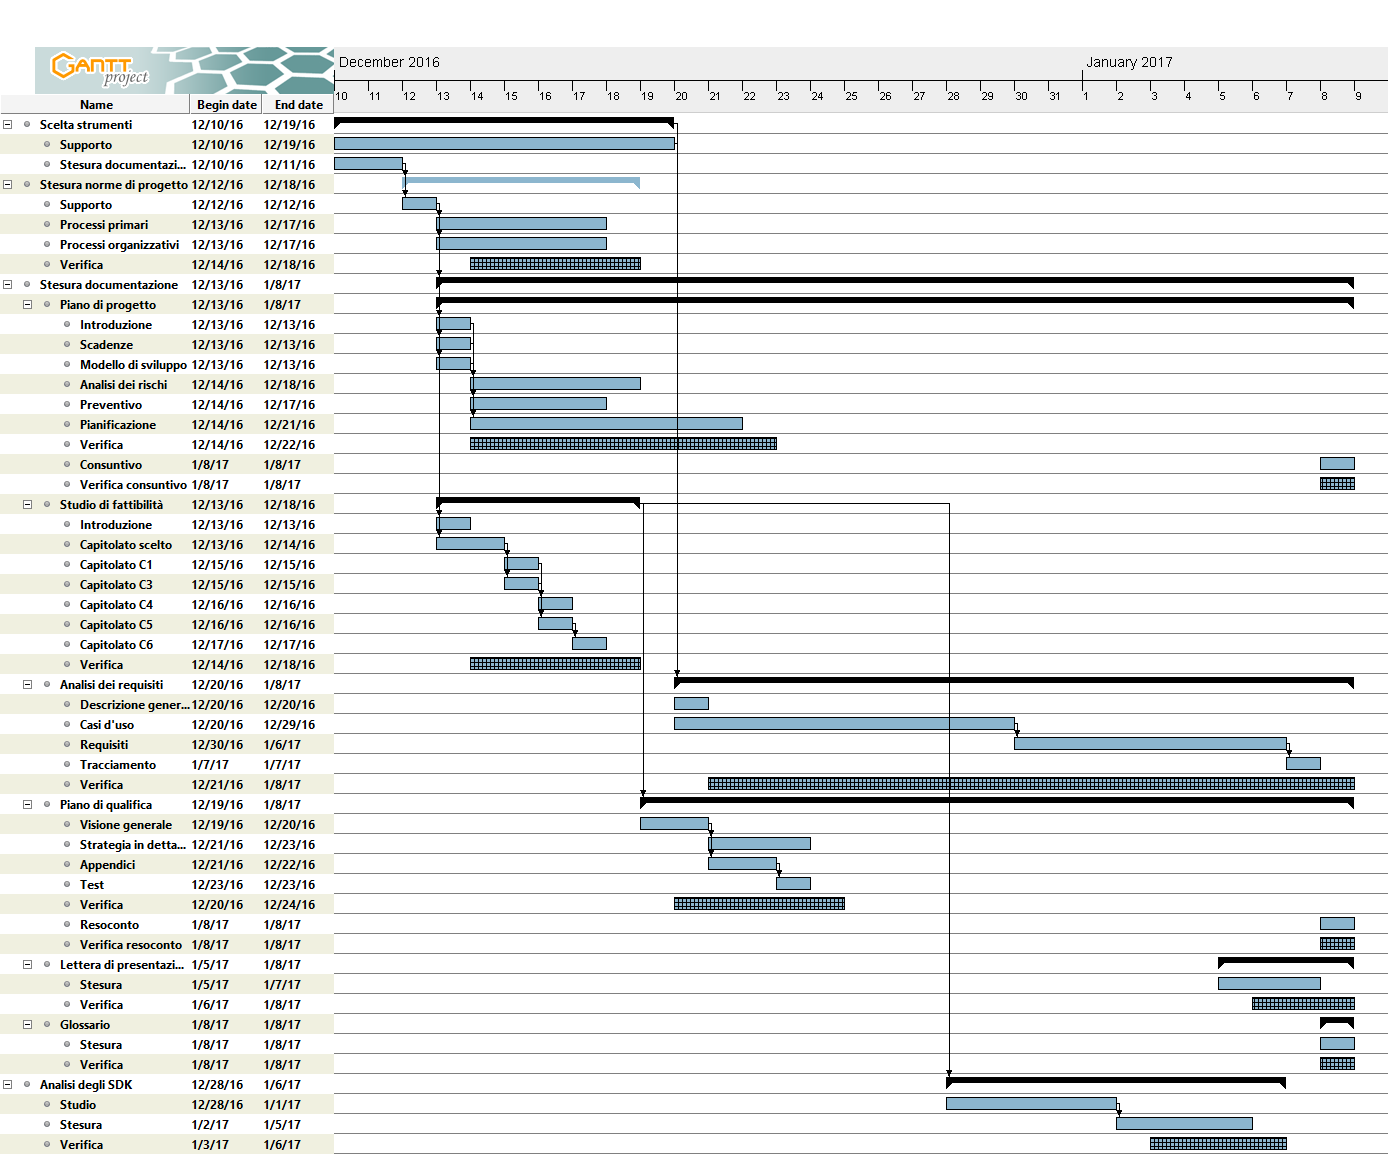
\includegraphics[width=\textwidth]{images/AR}
    \caption{Gantt - \PerAR}
    \end{figure}
    
	\subsection{\PerAD{} (AD)}
  \textbf{Periodo: dal 2017-01-24 al 2017-01-31}

  Questo periodo comincia al termine della \PerAR.  Le attività da svolgere in questo periodo saranno le seguenti:
  \begin{itemize}
    \item \textbf{Incremento e \gl{verifica} documenti}: tutti i documenti prodotti nel periodo precedente vengono incrementati e corretti in base alle segnalazioni del committente e del proponente;
    \item \textbf{Incremento e verifica requisiti}:  gli \ANP{} provvedono ad individuare nuovi requisiti e a correggere eventuali requisiti segnalati; tutti i documenti saranno aggiornati di conseguenza. Verrà fissato un incontro col proponente per la verifica dei requisiti individuati in questo modo.
    
    \clearpage
  \subsubsection{Diagramma di Gantt - \PerAD}
    \begin{figure}[!h]
    \centering
    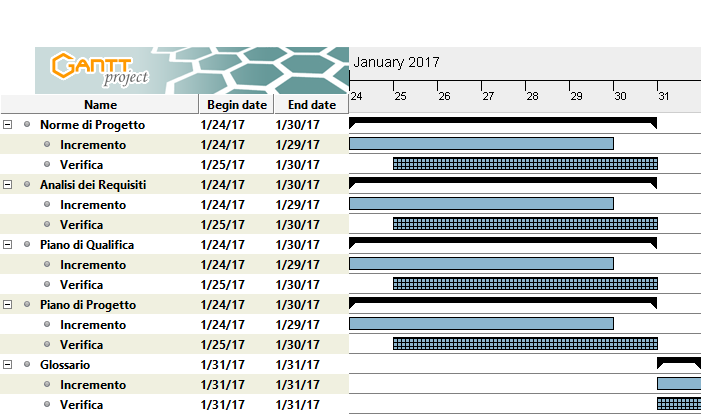
\includegraphics[width=\textwidth]{images/AD}
    \caption{Gantt - \PerAD}
    \end{figure}

  \subsection{\PerPA{} (PA)}
  \textbf{Periodo: dal 2017-02-01 al 2017-02-22}

  Questo periodo inizia al termine della \PerAD{} e termina con una \gl{milestone} interna di \label{Revisione} Progettazione minima. Al termine di questo periodo verrà fissato un incontro col proponente per presentare l'architettura logica prodotta. Le attività svolte durante questo periodo sono:
  \begin{itemize}
    \item \textbf{Incremento dei documenti}: dove necessario vengono apportate modifiche ai documenti già stilati, in preparazione alla  \textit{Specifica Tecnica};
    \item \textbf{Specifica Tecnica}: i \PJP{} effettuano le scelte progettuali atte allo sviluppo del \gl{prodotto}, definendo l'architettura generale del \gl{Software} che viene poi tracciata con i requisiti; il  tutto viene poi inserito nel documento \textit{Specifica Tecnica};
    \item \textbf{\gl{Verifica}}: viene effettuata la verifica sia dei documenti incrementati sia della \textit{Specifica Tecnica}.
  \end{itemize}

    %\item documentazione \gl{API}: viene prodotta una documentazione dettagliata delle varie API fornite dal \gl{sistema}};
    %\item piano di test di unità: viene creato il piano dei test di unità.
  \end{itemize}
\clearpage
  \subsubsection{Diagramma di Gantt - \PerPA}
    \begin{figure}[!h]
    \centering
    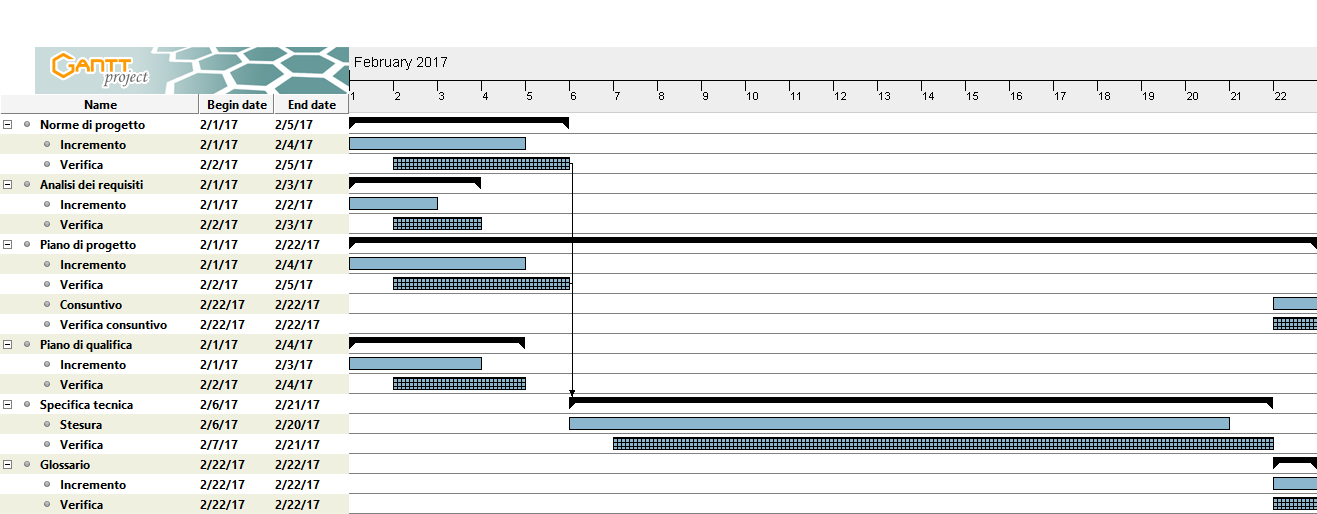
\includegraphics[width=\textwidth]{images/PA}
    \caption{Gantt - \PerPA}
    \end{figure}

  \subsection{\PerPD{} (PD)}
  \textbf{Periodo: dal 2017-02-27 al 2017-04-11}

  Questo periodo inizia con la fine della \PerPA{} e termina con la consegna dei documenti per la \textbf{Revisione di Progettazione} massima. Le attività che verranno svolte in questo periodo saranno:
  \begin{itemize}
    \item \textbf{Definizione di prodotto}: viene definita nel dettaglio la struttura interna del sistema e le relazioni tra i diversi moduli del prodotto, oltre ad una descrizione dettagliata di tutti le API del sistema; il tutto viene riportato nel documento \DPdocRP.
    \item \textbf{Piano dei test}: viene definito un piano dei test di unità, integrazione e sistema atto alla verifica e \gl{validazione} delle componenti del sistema; esso viene inserito nel \PQdocRP{};
    \item \textbf{Incremento e verifica dei documenti}: se ritenuto necessario vengono apportate modifiche ai documenti già stilati.
  \end{itemize}
\newpage
  \subsubsection{Diagramma di Gantt - \PerPD}
    \begin{figure}[!h]
    \centering
    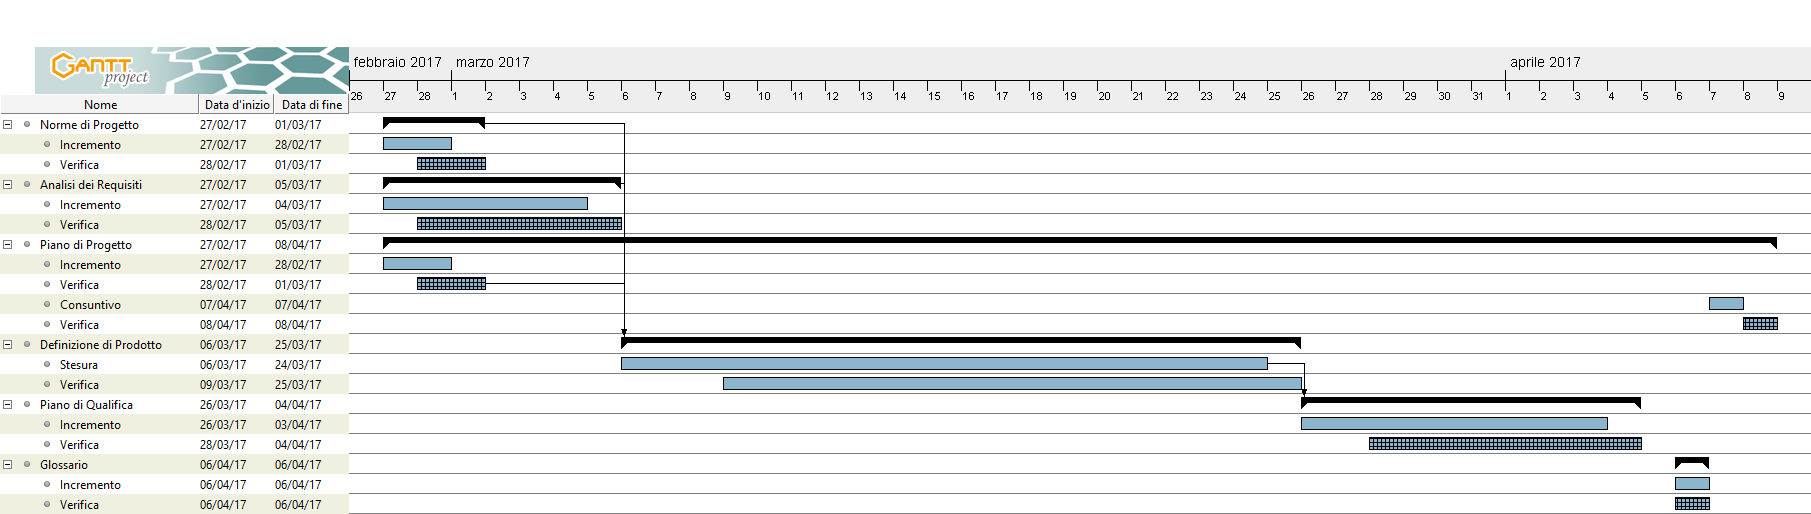
\includegraphics[width=\textwidth]{images/PD}
    \caption{Gantt - \PerPD}
    \end{figure}

  \subsection{\PerC{} (C)}
  \textbf{Periodo: dal 2017-04-18 al 2017-05-07}

  Questo periodo inizia in seguito all'esito della \textbf{Revisione di Progettazione} e termina con la consegna del prodotto alla \textbf{Revisione di Qualifica}. Le attività svolte saranno:
  \begin{itemize}
    \item \textbf{Codifica}: in base a quanto definito nel documento di \textit{Definizione di \gl{Prodotto}}, i \PRP{} sviluppano il codice del prodotto \gl{software}. Si divide in codifica obbligatoria, desiderabile ed opzionale in base all'utilità strategica dei requisiti che vengono soddisfatti dal codice prodotto. A seconda del tempo impiegato dalla codifica obbligatoria, il tempo previsto per codifica desiderabile ed opzionale potrebbe essere ridotto parzialmente o totalmente.
    \item \textbf{Test}: contemporaneamente all'inizio della codifica del sistema, si inizia la stesura dei test di unità, integrazione e sistema come previsto nel \textit{Piano di Qualifica};
    \item \textbf{Automazione}: gli \AMMP{} si occuperanno della predisposizione di sistemi automatizzati per l'esecuzione automatica dei test.
    \item \textbf{Manuale utente}: verrà steso il \textit{Manuale Utente}, destinato agli utilizzatori finali del sistema.
  \end{itemize}

  \newpage
  \paragraph{Diagramma di Gantt - \PerC}
    \begin{figure}[!h]
    \centering
    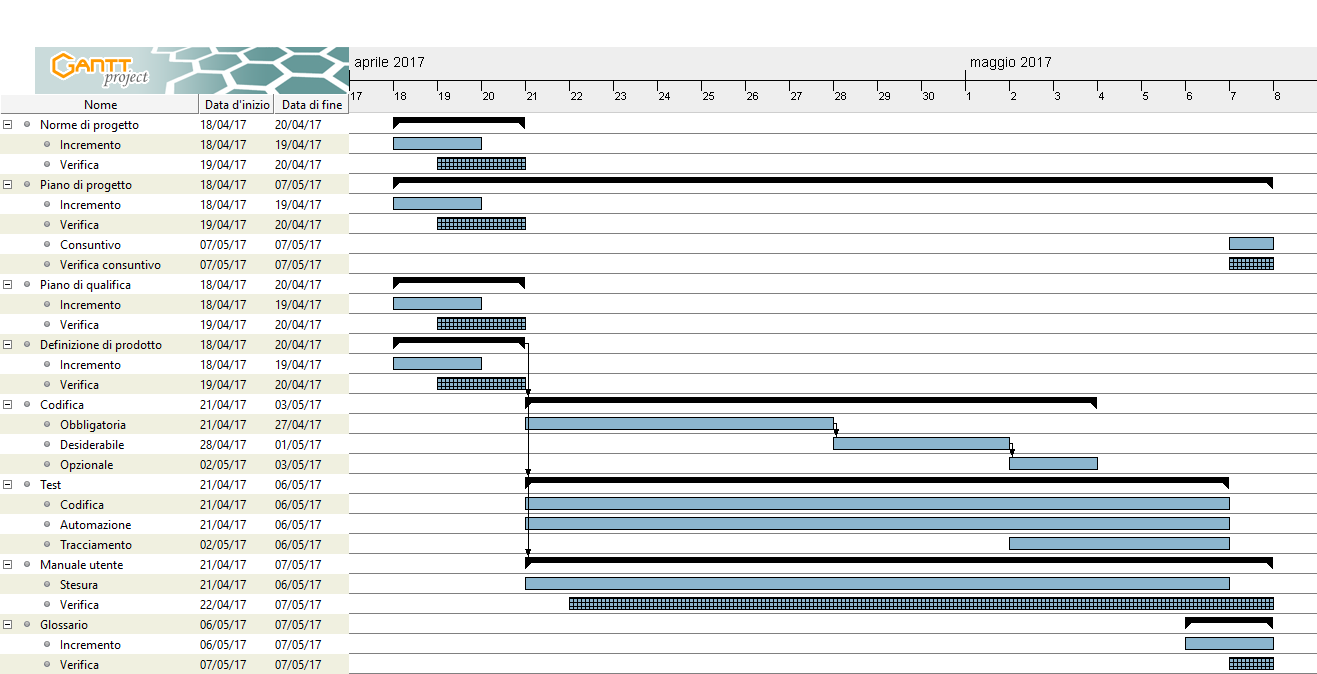
\includegraphics[width=\textwidth]{images/C}
    \caption{Gantt - \PerC}
    \end{figure}

  \subsection{\PerV (V)}
  \textbf{Periodo: dal 2017-05-15 al 2017-06-10}

  Questo periodo inizia dopo l'esito della \textbf{Revisione di Qualifica} e termina con la consegna della \textbf{Revisione d'Accettazione}. Le attività che verranno svolte saranno:
  \begin{itemize}
    \item \textbf{Incremento e verifica} dei documenti: se ritenuto necessario vengono apportate modifiche ai documenti già stilati;
    \item \textbf{\gl{Validazione}}: viene verificato, con l'aiuto del tracciamento, di aver soddisfatto i requisiti presenti nel documento \textit{Analisi dei Requisiti};
    \item \textbf{Esecuzione test}: si continua l'esecuzione dei test di unità, integrazione e sistema codificati ed eseguiti nei periodi precedenti;
    \item \textbf{Correzione bug}: vengono tracciati e risolti i bug rilevati;
    \item \textbf{Collaudo}: si esegue un collaudo completo del sistema creato.
  \end{itemize}

 \newpage
  \subsubsection{Diagramma di Gantt - \PerV}
    \begin{figure}[!h]
    \centering
    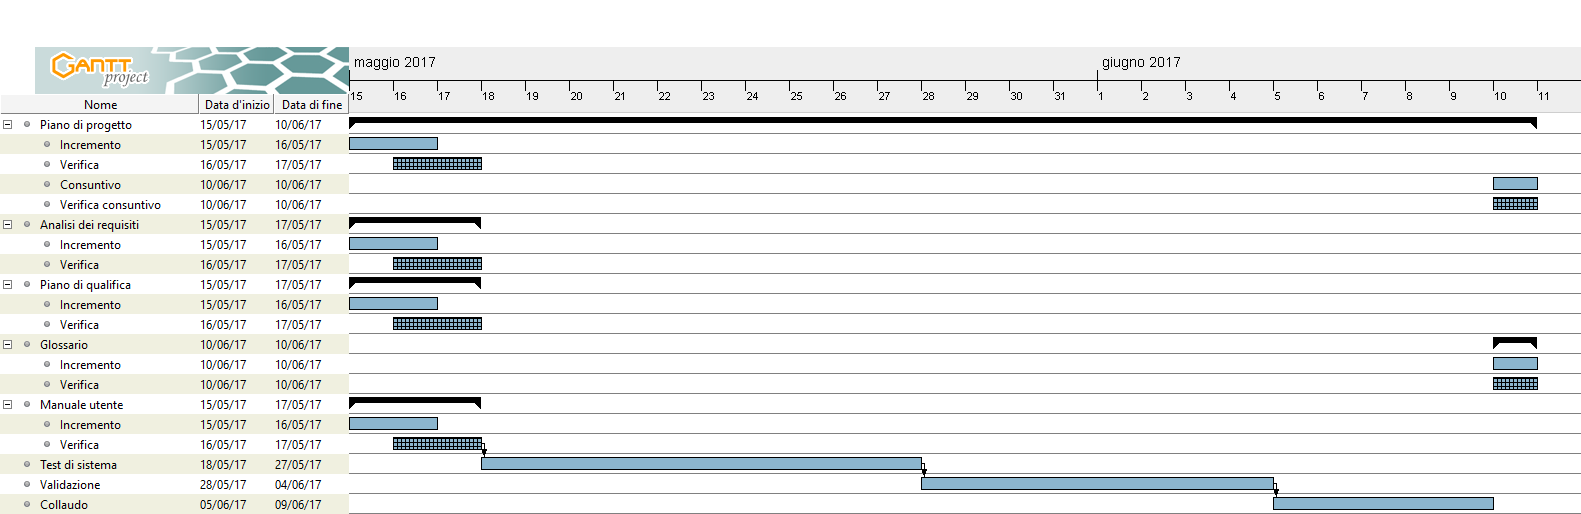
\includegraphics[width=\textwidth]{images/V}
    \caption{Gantt - \PerV}
    \end{figure}
\end{document}
